\documentclass[margin]{res}
\usepackage{graphicx}
\usepackage{tabu}
\usepackage{multirow}

%\usepackage{helvetica} % uses helvetica postscript font (download helvetica.sty)
%\usepackage{newcent}   % uses new century schoolbook postscript font 
\setlength{\textwidth}{5.1in} % set width of text portion
\renewcommand{\arraystretch}{1.2}

\begin{document}

% Center the name over the entire width of resume:
 \moveleft.5\hoffset\centerline{\Large\bf Deval Srivastava}
% Draw a horizontal line the whole width of resume:
 \moveleft\hoffset\vbox{\hrule width\resumewidth height 1pt}\smallskip
\hskip-3.0cm\begin{tabular*}{6in}{l@{\extracolsep{\fill}}r}
        & \multirow{1}{*}{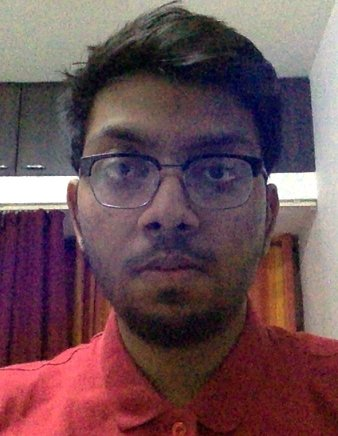
\includegraphics[scale=0.27]{profile}}\\
         
        %-----------------------------------------------------------  
        Army Colony, Nerul & \\
        Navi Mumbai-400706  \\
        Maharashtra\\
        dex345z@gmail.com \\
        9699727877\\
    \end{tabular*}

\begin{resume}
 
 \section{OBJECTIVE} To obtain an internship that will allow me to utilize my problem solving and analytical skills to further develop my abilities in the field of computer science.\\

\section{EDUCATION}\begin{tabu} to 1\textwidth { | X[c] | X[c] | X[c] | X[c]| X[c]|}
 \hline
 Degree & College /School & University & Passing Year & Pass Percentage\\
 \hline
 BE. Info Tech. & Fr.CRCE &Mumbai University & 2019 & 7.8 (Till Sem V) \\
\hline
HSC & DPS (Navi Mumbai)& CBSE & 2015 & 92.8\\
\hline
SSC & DPS (Navi Mumbai) & CBSE & 2013 & 9.4 GPA\\
\hline
\end{tabu}

\section{PROJECTS } \begin{enumerate}
  \item  {\large{\sl Automated Traffic Surveillance System}}\\
 Built a complete end-to end system which detects real time road offences and send the vehicle plate data to a database/website, we utilised the FR-CNN object detection model and various image processing techniques.\\
        - implemented the license plate extractor algorithm using morphological operations and other operations in opencv individually.\\
        -Developed the complete website using NodeJs which employed sockets to display offences in real time. Integrated maps in the application to monitor the physical location of the offence. Wrote python Script to pipeline data to the website after parsing and encoding
 \item {\large{\sl Activity Detection and Facial Recognition}}\\
 Developed a system to recognise the face of a person if human activity was detected and then log data to a database.\\
  	-Implemented the activity detector using background subtraction and detected Faces using haar cascades.\\
	-Recognised faces utilising the facenet neural network trained on CASIA-WebFace dataset.Image along with the identified name were stored in the database\\
	-Built using Opencv and Tensorflow in python.\\
	\end{enumerate}

\section{INTERNSHIPS} \begin{itemize}
 \item{\large{\sl Software Developer Intern at Freeways}}\hfill 2017 \\
 	Interned for an early stage tourism startup worked on their backend and databases.\\
	-Reformatted the database and removed noisy data.\\
	-Developed their admin panel to enable high level access to the database.\\
	-Built a Rest API which  provided locations  based on ratings received.\\
	-Languages and frameworks used Nodejs , MongoDB and React.\\
 \end{itemize}

\section{TRAINING}\begin{itemize}
 \item{\sl  "Fast.ai" course by jeremy howard }
 \item{\sl  "Intro to computer vision " course by Udacity}
 \item{\sl  "intro to machine learning" course by Udacity}
 \end{itemize}

\section{TECHNICAL  \\ SKILLS} \begin{enumerate}
\item {\sl Programming Langauges \& Scripts }\\
	-Python,Nodejs,JavaScript,JAVA, Bash, basic c/c++
\item {\sl Frameworks \& Libraries}\\
	-Tensorflow, Opencv, Pytorch,matploitlib
\item {\sl Web Technologies}\\
	-ReactJs,REST,MEAN,HTML5, CSS3, SemanticUI
\item{\sl Databases}\\
	-MongoDB,MySQL,PostgreSQL,AWS DynamoDB
\end{enumerate}

\section{SOFT SKILLS }\begin{enumerate}
\item{\sl Decision Making}
\item{\sl Adapt to new situations quickly}
\item{\sl Conflict Resolution.}
\item{\sl Good team player.}
\end{enumerate}


\section{EXTRA CURRICULAR ACTIVITIES}\begin{itemize}
\item{\sl Technical Head at CSI(Computer Society India) chapter of Fr.Crce}
\item{\sl Participated in State Level Hackathon err404}
\item{\sl Participated in National level Project Competition}
\end{itemize}


\section{PERSONAL INFORMATION}
{\sl Father's Name:} Arvind Srivastava\\
{\sl Mother's Name:} Madhu Srivastava\\
{\sl Sex:} Male\\
{\sl Date of Birth:} 24th October 1997\\
{\sl Nationality:} Indian\\
{\sl Maritial Status:} Unmarried\\

\section{DECLARATION} 
{\sl I here by declare that the above information is true and best of my knowledge}

 \section{DATE}
 {\sl : 17th April 2018}

\end{resume}
\end{document}




